%%%%%%%%%%%%%%%%%%%%%%%%%%%%%%%%%%%%%%%%%
% Beamer Presentation
% LaTeX Template
% Version 1.0 (10/11/12)
%
% This template has been downloaded from:
% http://www.LaTeXTemplates.com
%
% License:
% CC BY-NC-SA 3.0 (http://creativecommons.org/licenses/by-nc-sa/3.0/)
%
%%%%%%%%%%%%%%%%%%%%%%%%%%%%%%%%%%%%%%%%%

%----------------------------------------------------------------------------------------
%	PACKAGES AND THEMES
%----------------------------------------------------------------------------------------
\documentclass[10pt]{beamer}

\usebackgroundtemplate%

\mode<presentation> {

% The Beamer class comes with a number of default slide themes
% which change the colors and layouts of slides. Below this is a list
% of all the themes, uncomment each in turn to see what they look like.

%\usetheme{default}
%\usetheme{AnnArbor}% yellow headings?
%\usetheme{Antibes}
%\usetheme{Bergen}
%\usetheme{Berkeley}
%\usetheme{Berlin}
\usetheme{Boadilla}
%\usetheme{CambridgeUS}
%\usetheme{Copenhagen}
%\usetheme{Darmstadt}
%\usetheme{Dresden}
%\usetheme{Frankfurt}
%\usetheme{Goettingen}
%\usetheme{Hannover}
%\usetheme{Ilmenau}
%\usetheme{JuanLesPins}
%\usetheme{Luebeck}
%\usetheme{Madrid}%my general fav
%\usetheme{Malmoe}
%\usetheme{Marburg}
%\usetheme{Montpellier}
%\usetheme{PaloAlto}
%\usetheme{Pittsburgh}
%\usetheme{Rochester}
%\usetheme{Singapore}
%\usetheme{Szeged}
%\usetheme{Warsaw}

% As well as themes, the Beamer class has a number of color themes
% for any slide theme. Uncomment each of these in turn to see how it
% changes the colors of your current slide theme.

%\usecolortheme{albatross}
%\usecolortheme{beaver}
%\usecolortheme{beetle}
%\usecolortheme{crane}
%\usecolortheme{dolphin}
%\usecolortheme{dove}
%\usecolortheme{fly}
%\usecolortheme{lily}
%\usecolortheme{orchid}
%\usecolortheme{rose}
%\usecolortheme{seagull}
\usecolortheme{seahorse}
%\usecolortheme{whale}
%\usecolortheme{wolverine}

%\setbeamertemplate{footline} % To remove the footer line in all slides uncomment this line
%\setbeamertemplate{footline}[page number] % To replace the footer line in all slides with a simple slide count uncomment this line

%\setbeamertemplate{navigation symbols}{} % To remove the navigation symbols from the bottom of all slides uncomment this line
}

\usepackage{graphicx} % Allows including images
\usepackage{booktabs}
\usepackage{movie15} % Allows the use of \toprule, \midrule and \bottomrule in tables


%----------------------------------------------------------------------------------------
%	TITLE PAGE
%----------------------------------------------------------------------------------------
\setbeamertemplate{navigation symbols}{} %turn off navigation symbols
\title[Hydrogen Refueling Techniques]{Thermodynamic Modelling: Hydrogen Refuelling Station} % The short title appears at the bottom of every slide, the full title is only on the title page

\author[Jerin Roberts]{Jerin Roberts, Dr. Walter M\'{e}rida, Dr. Omar Herrera} % Your name

\institute[University of British Columbia] % Your institution as it will appear on the bottom of every slide, may be shorthand to save space
{


}
\date{\today} % Date, can be changed to a custom date

\begin{document}
\centering\usebackgroundtemplate{
\includegraphics[width=12.65cm]{back1}}%

\begin{frame}
\centering

\titlepage % Print the title page as the first slide
%
\includegraphics[width=1.5cm]{ubc}
\end{frame}
\usebackgroundtemplate{
\includegraphics[width=12.80cm]{back2}}
\begin{frame}
\frametitle{Overview} % Table of contents slide, comment this block out to remove it
\tableofcontents % Throughout your presentation, if you choose to use \section{} and \subsection{} commands, these will automatically be printed on this slide as an overview of your presentation
\end{frame}

%----------------------------------------------------------------------------------------
%	PRESENTATION SLIDES
%----------------------------------------------------------------------------------------

%------------------------------------------------
\section{Overview} % Sections can be created in order to organize your presentation into discrete blocks, all sections and subsections are automatically printed in the table of contents as an overview of the talk
%------------------------------------------------

 % A subsection can be created just before a set of slides with a common theme to further break down your presentation into chunks



\begin{frame}
\frametitle{explanation}
\begin{columns}
\begin{column}{0.5\textwidth}
   \frametitle{Why Hydrogen Fuel?}
     \begin{itemize}
      \item High specific energy content
      \item Relatively Abundant
      \item Low Emissions
      \end{itemize}
      
      \begin{center}
     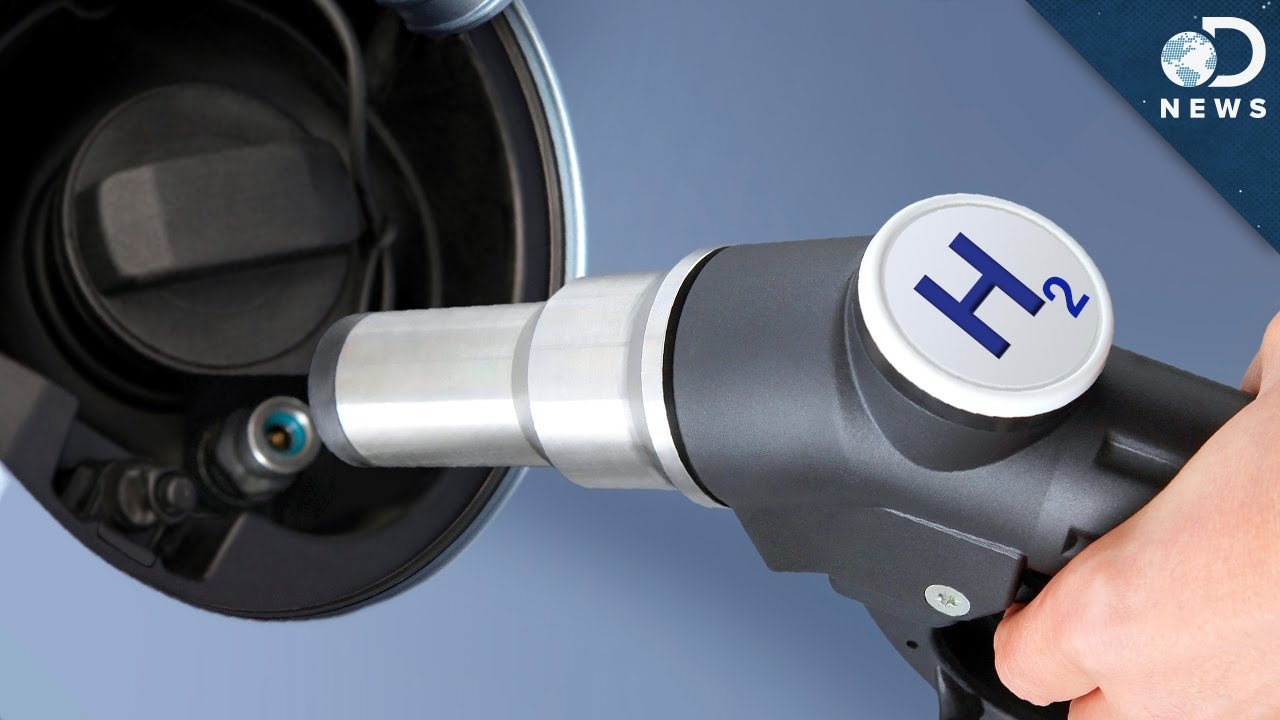
\includegraphics[width=0.9\textwidth]{noz.jpg}
     \end{center}
\end{column}
\begin{column}{0.5\textwidth}  %%<--- here
    \begin{center}
     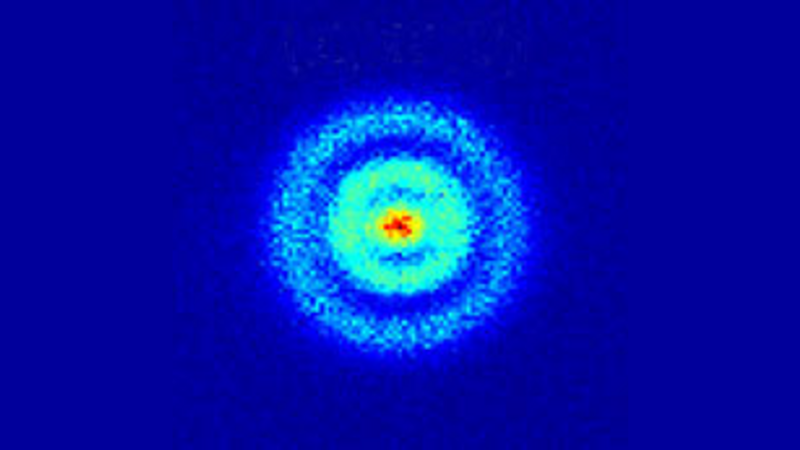
\includegraphics[width=0.9\textwidth]{hyd}
     \end{center}
     
     \begin{itemize}
      \item Infrastructure Integration
      \item Simple Production
      \item Relatively Renewable 
      \end{itemize}
\end{column}
\end{columns}
\end{frame}

%------------------------------------------------
\section{Storage Types}
\begin{frame}{ubc}
\frametitle{Hydrogen Storage}
Can be stored in Liquid or Gaseous States
 

     
\begin{itemize}
\item Liquid Hydrogen Has very high Energy Density
\item Gaseous Hydrogen uses cheap and simple storage 
\end{itemize}
     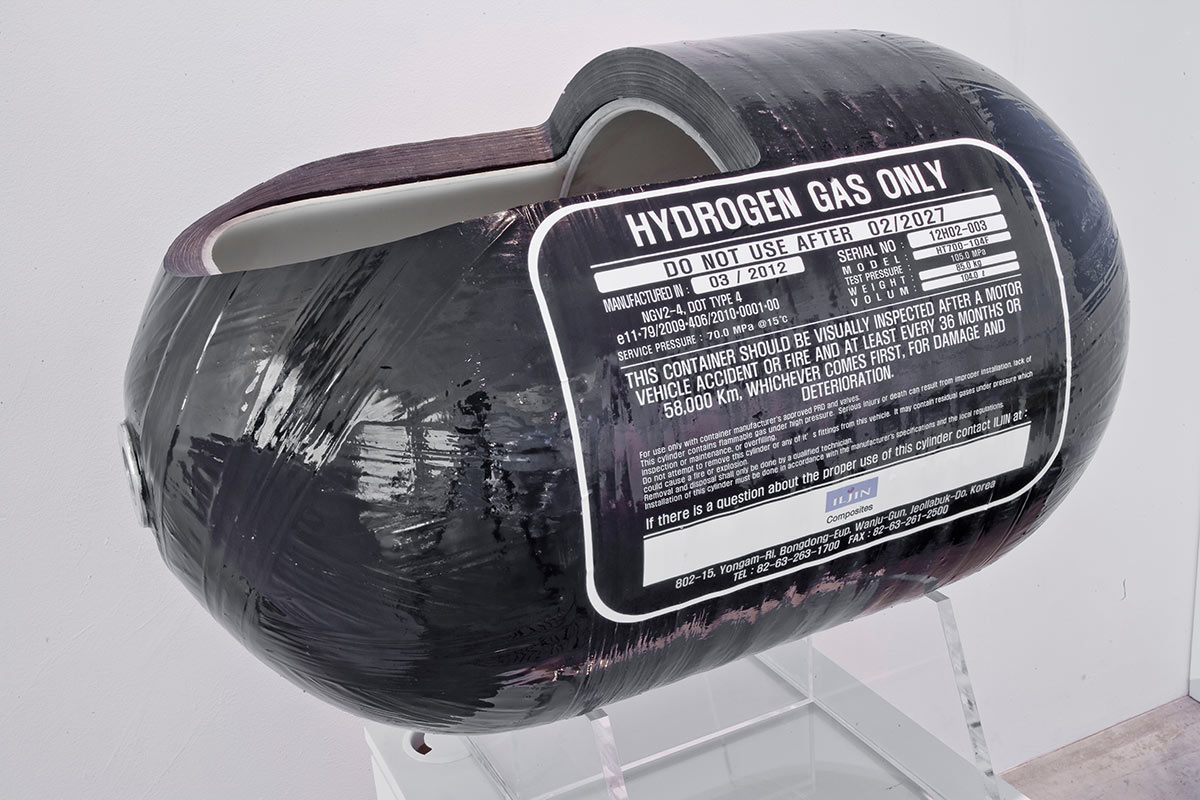
\includegraphics[height=0.22\textwidth]{htank}
          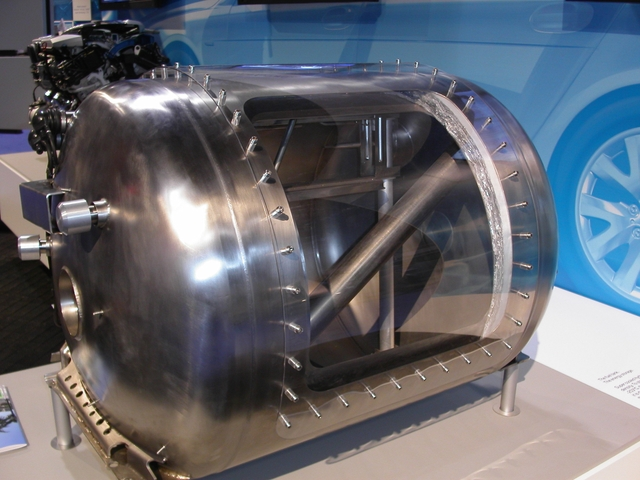
\includegraphics[height=0.22\textwidth]{liq}
\begin{itemize}
\item Liquid Requires Complex Cryogenic Systems
\item Gaseous Hydrogen Has to be Compressed to match acceptable energy density 
\end{itemize}

\end{frame}

\section{Modeling}
\begin{frame}
\frametitle{Modelling Temperature Distribution}
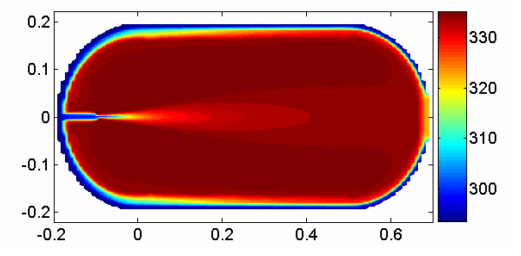
\includegraphics[height=0.4\textwidth]{mod1}

Temperature Distribution for 35MPa Tank during fast filling \cite{p2}
\end{frame}
%------------------------------------------------
\section{Metrics}
\begin{frame}
\frametitle{Problem and Constraints}
\begin{itemize}

\item  Map 2D temperature distribution inside tank

\item Determine mass transfer during a fast fill.

\item  Determine Pressure during fast fill

\item  Semi-portable system

\item  No modifications to tank

\item  Adhere to SAEJ2601 standards

\end{itemize}
\end{frame}



%------------------------------------------------


\section{Experimental System}

\begin{frame}{ubc}
\frametitle{Experimental Setup}

\center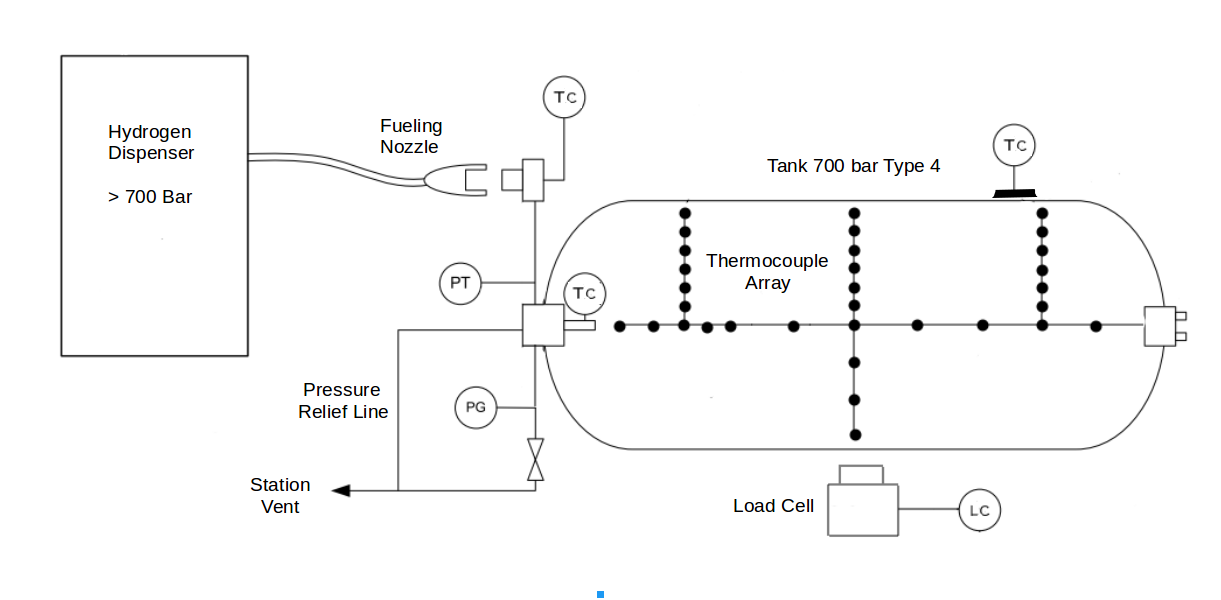
\includegraphics[height=6cm]{schem2}
\end{frame}
%------------------------------------------------

\begin{frame}{ubc}
\frametitle{Data Acquisition System}

\center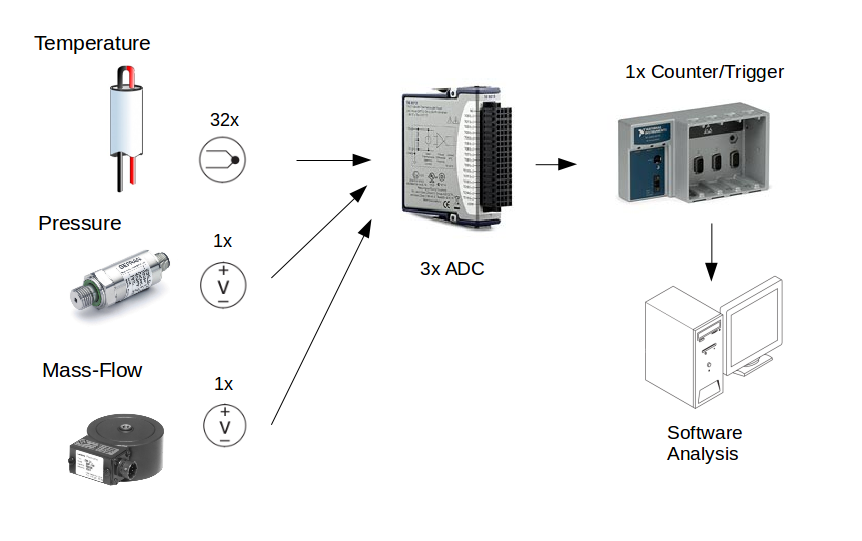
\includegraphics[height=6cm]{sch.png}
\end{frame}


%------------------------------------------------


\section{Sensors}
\begin{frame}


\begin{columns}
\begin{column}{0.5\textwidth}
  \frametitle{Temperature}
Thermocouple:
 \begin{center}
     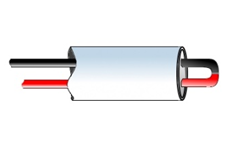
\includegraphics[width=0.6\textwidth]{Therm}
     \end{center}
\begin{itemize}
\item Type T Special Grade
\item 0.012mm Diameter $\tau = 0.4$ s
\item $\pm 0.5^{\circ}$C accuracy

\end{itemize}
\end{column}
\begin{column}{0.5\textwidth}  %%<--- here
  ADC 2x NI 9213 
     
     \begin{itemize}
      \item 16ch 24 bit ADC
      \item $\pm$78.125mV input range @ 78 S/s
      \item accuracy with type T $\pm 0.02^{\circ}$C
      \end{itemize}
      
       \begin{center}
     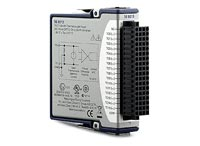
\includegraphics[width=0.5\textwidth]{adc}
     \end{center}
\end{column}
\end{columns}
\end{frame}

%------------------------------------------------


\section{Sensors}
\begin{frame}


\begin{columns}
\begin{column}{0.5\textwidth}
  \frametitle{Temperature}
Thin-Film Heat Flux Sensor:
 \begin{center}
     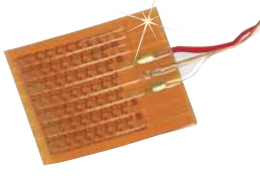
\includegraphics[width=0.6\textwidth]{film}
     \end{center}
\begin{itemize}
\item Type K Standard Grade
\item $\tau = 1.5$ s
\item $\pm 1.1^{\circ}$C accuracy

\end{itemize}
\end{column}
\begin{column}{0.5\textwidth}  %%<--- here
  ADC 2x NI 9213 
     
     \begin{itemize}
      \item 16ch 24 bit ADC
      \item $\pm$78.125mV input range @ 78 S/s
      \item accuracy with type T $\pm 0.02^{\circ}$C
      \end{itemize}
      
       \begin{center}
     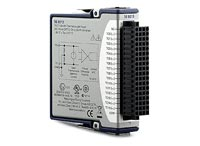
\includegraphics[width=0.5\textwidth]{adc}
     \end{center}
\end{column}
\end{columns}
\end{frame}


%------------------------------------------------

\begin{frame}


\begin{columns}
\begin{column}{0.5\textwidth}
  \frametitle{Pressure}
GEFRAN Diaphragm Transducer:
 \begin{center}
     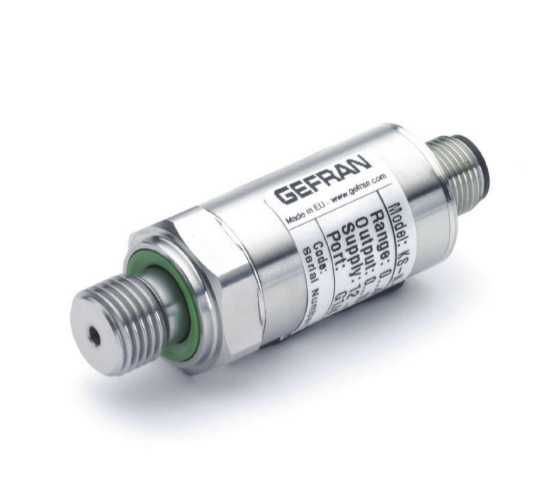
\includegraphics[width=0.5\textwidth]{press}
     \end{center}
\begin{itemize}
\item 0-1000 Bar for 0-10V
\item Response Time $\leq$ 1msec
\item $\pm 0.5\%$ accuracy FS

\end{itemize}
\end{column}
\begin{column}{0.5\textwidth}  %%<--- here
   
  ADC 1x NI 9215 
     
     \begin{itemize}
      \item 4ch 16 bit ADC
      \item $\pm$10V input range @ 100 kS/s
      \item $\leq 0.2\%$ error (calibrated)
      \end{itemize}
      
       \begin{center}
     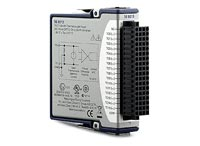
\includegraphics[width=0.65\textwidth]{adc}
     \end{center}
\end{column}
\end{columns}
\end{frame}

%------------------------------------------------

\begin{frame}


\begin{columns}
\begin{column}{0.5\textwidth}
  \frametitle{Mass Flow}
Honeywell 3397 Load cell:
 \begin{center}
     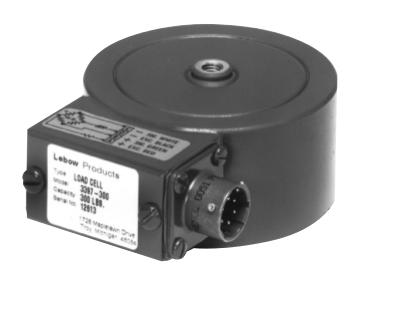
\includegraphics[width=0.4\textwidth]{load}
     \end{center}
\begin{itemize}
\item 2mV/V $\pm 0.25\%$ 
\item 0-200lb range
\item Universal Inline Amplifier $\pm$10Vdc

\end{itemize}
\end{column}
\begin{column}{0.5\textwidth}  %%<--- here
   
  ADC 1x NI 9215 
     
     \begin{itemize}
      \item 4ch 16 bit ADC
      \item $\pm$10V input range @ 100 kS/s
      \item $\leq 0.2\%$ error (calibrated)
      \end{itemize}
      
       \begin{center}
     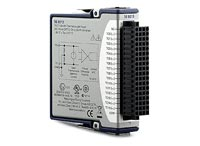
\includegraphics[width=0.5\textwidth]{adc}
     \end{center}
\end{column}
\end{columns}
\end{frame}

\section{Experimental Protocol}

\begin{frame}
\frametitle{Procedure}
\begin{itemize}
\item Purge Tank and Set Pressure to 50 Bar
\item Allow Temperature/Pressure to Stabilize 
\item Record Initial Conditions
\item Apply Required Ramp Rate
\item Measure P, T @ 20S/s HF, m @ 1S/s during Fast fill
\item Measure P, T @ 20S/s HF, m @ 1S/s during cool down
\item Record Final Conditions
\item Repeat for different array configurations
\end{itemize}
\end{frame}



%------------------------------------------------
\section{Summary}
\begin{frame}
\frametitle{Summary}
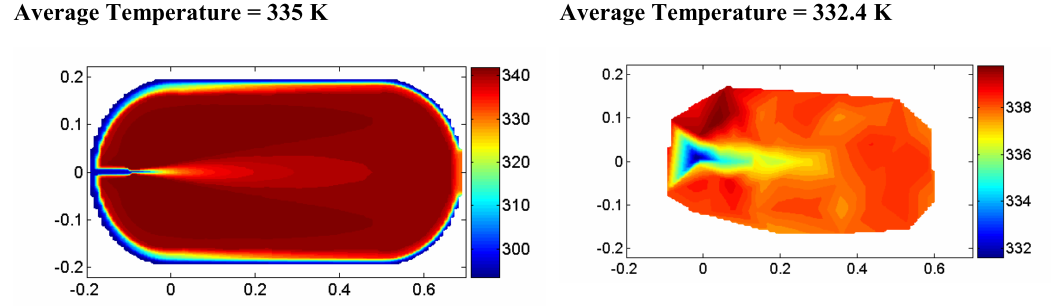
\includegraphics[height=0.25\textwidth]{fin}




\begin{itemize}
      \item Temperature: T $\pm$0.16$\%$
      \item Pressure: P $\pm$0.22$\%$
      \item Heat Flux: HF $\pm$0.4$\%$
      \item Mass: m $\pm$0.45$\%$
      \end{itemize}
\end{frame}



\begin{frame}
\frametitle{References}
\footnotesize{
\begin{thebibliography}{99} % Beamer does not support BibTeX so references must be inserted manually as below
\bibitem[Rothuizen, 2013]{p1} Rothuizen, Erasmus Damgaard; Rokni, Masoud; Elmegaard, Brian (2013)
\newblock "A Thermodynamic Analysis of Fuelling Hydrogen Vehicles for Personal Transportation" Technical University of Denmark
\newblock Nils Koppels Allé, Bldg. 403 DK-2800 Kongens Lyngby Denmark


\bibitem[Dicken, 2006]{p2} Dicken, Chris;(2006)
\newblock "Temperature Distribution within a Compressed Gas Cylinder during Fast Filling"
\newblock  Advanced Materials Research, Vols. 15-17, pp. 281-286, 2007 


\bibitem[Hirotani et al, 2006]{p3} Hirotani, R.
Tomioka, J. ;Maeda, Y. ;Mitsuishi, H. ;Watanabe, S.;(2006)
\newblock "Thermal Behavior in Hydrogen Storage Tank for Fuel Cell Vehicle on Fast Filling"
\newblock  Proceedings of the 16th World Hydrogen Energy Conference, 13-16 June 2006, Lyon (France)

\end{thebibliography}
}
\end{frame}

%------------------------------------------------

\begin{frame}

\large\centerline{Thank-you}

\small
\end{frame}

%----------------------------------------------------------------------------------------


\end{document} 